\chapter{Problemas Abordados}
\label{ch:problemas}
Nessa seção será apresentada uma breve introdução aos \textit{benchmarks} que serão utilizados para análise nesse trabalho, junto a isso é feito uma introdução aos problemas dinâmicos, suas variações e dificuldades.

Durante o dia a dia, pode-se observar diversos problemas complexos em que as condições do ambiente podem mudar com o passar do tempo, sendo assim uma solução válida com o passar do tempo, acaba não sendo mais suficientemente boa para suprir as necessidades das novas condições \cite{branke2012evolutionary}.Para problemas com mudanças em seu ambiente é necessário um sistema de resolução que se adapte as alterações e esteja sempre apto a procurar por soluções melhores.

Na computação existem várias áreas que se dedicam a otimizar problemas desse tipo como por exemplo os EA e os IS. Para que poder avaliar os algoritmos utilizados na otimização destes problemas são geradas funções \textit{benchmarks} que apresentam características dos problemas reais, como por exemplo mudança de elevação de terrenos.

\section{Funções \textit{Benchmark}}
\label{sec:revisao_benchmark}
O uso das funções \textit{benchmark} é um ponto crucial para o desenvolvimento, comparação, avaliação e otimização dessa classe de problemas \cite{evolution_dynamic}. O fato das condições do problema variarem de acordo com o tempo acrescentam uma camada de dificuldade a mais para obter uma solução satisfatória após uma mudança. Um bom \textit{benchmark} possui as seguintes características.

\begin{enumerate}  
\item Flexibilidade: Configurável sobre diferentes abordagens dinâmicas, como por exemplo, a frequência ou intensidade das alterações no ambiente, em diferentes escalas.

\item Simplicidade e Eficiência: Deve ser fácil de implementar e analisar.

\item Associação com Problemas Reais: Ter a capacidade de fazer previsões em problemas reais ou se assemelhar em alguma extensão.
\end{enumerate}

Para a analisar um \textit{benchmarks} é necessário dar atenção para o tipo de dinamismo que esse problema apresenta, pois para otimiza-lo são escolhidas estratégias de otimização baseadas no tipo de dinamismo. Cada \textit{benchmarks} possui suas características e com isso cada algoritmo aplicado a ele terá que analisar como está abordando essas peculiaridades. A Características observadas nas funções encontradas são \cite{cruz2011optimization}:

\begin{enumerate}
\item Influência Temporal: Sempre que uma solução futura depende de outra encontrada anteriormente pelo algoritmo, ou seja, quando o tipo de mudança que o algoritmo vai sofrer depende de quais soluções foram encontradas ao decorrer da otimização. Neste caso os resultados podem mudar para cada tentativa de otimização.

\item Previsibilidade: Quando as mudanças geradas pelo problema seguem um padrão que pode ser previsto durante a otimização do problema. Podem ser alterações por mudança em uma escala fixa, incremental, cíclica, periódica.

\item Visibilidade: Sempre que as mudanças são visíveis pelo algoritmo que está otimizando o problema, de foram que o algoritmo não precise usar muitos detectores para perceber a mudança no ambiente. Podem ser pontos específicos do espaço, que são detectados ao re-avaliar a função objetivo, ou até mesmo, as restrições.

\item Problemas com Restrições: As mudanças do problema podem ocorrer nas restrições, que podem mudar ao longo do tempo (a variável de tempo influencia na função de restrição) ou o podem ser ativadas e/ou desativadas durante a otimização.

\item Número de Objetivos: São as problemas multi-objetivos, que neste caso podem alterar o número de objetivos durante a otimização, chegando até, ao ponto de tem somente um objetivo em vista.

\item Intensidade das Mudanças: qual a escala da mudança, ou qual o período de ciclo das mudanças, ou o limite das mudanças.

\item Fator da Mudança: Onde o dinâmismo pode ocorrer, sendo: Função objetivo; Domínio das variáveis; Número de variáveis; Restrições; ou outros parâmetros.  
\end{enumerate}

\subsection{Avaliação de Desempenho}
\label{sec:perfermance_measures}

Para avaliar um \textit{benchmarks} são estipuladas métricas que serão utilizadas para medir a qualidade dos resultados obtidos pelo algoritmo de otimização. Os métodos de avaliação apresentados foram selecionados por serem amplamente utilizados em algoritmos bioinspirados aplicados em ambientes dinâmicos e possivelmente serão usados para avaliar o desempenho dos algoritmos selecionados neste trabalho.
A forma de avaliação pode ser dividida em dois grandes grupos: Medida de desempenho baseados em otimalidade e os em comportamento.

\subsubsection{Otimalidade}
As medidas de desempenho baseadas na otimalidade avaliam a capacidade dos algoritmos em encontrar as soluções com o melhor valor de \textit{fitness} ou as que estão mais próximas do ótimo global (medidas baseadas na distância) e essa avaliação leva em conta o algoritmo como um todo. Entre elas tem-se:

\begin{itemize}
\item Melhor da Geração: Avalia qual o melhor indivíduo de cada iteração do algoritmo, gerando assim uma curva de desempenho que apresenta os pontos de melhora do algoritmo e o quão perto está do ótimo do problema. Esse é o método mais frequentemente utilizado.

\item Melhor Erro Antes da Mudança: Calcula a média do erro (diferença da melhor solução atual para o ótimo do problema) da população logo antes da mudança do ambiente. Este caso só pode ser usado quando o dinamismo do \textit{benchmark} gerado é previsível ou facilmente identificável, que por sua vez, dependo de como o \textit{benchmark} muda o ambiente.

\item Pontuação Normalizada: Mede a diferença entre uma determinada gama de algoritmos em relação a uma lista pré-determinada de problemas, fazendo com que cada algoritmo execute cada problema um número determinado de vezes. Com os resultados normalizados, para a melhor solução é atribuído o valor 1(um) e para a pior solução é atribuído o valor 0(zero).
\end{itemize}

\subsubsection{Comportamento}
As medidas de desempenho baseadas em comportamento avaliam a influência de certos comportamentos que são importantes na hora de manter um nível de \textit{fitness}, como por exemplo:

\begin{itemize}
\item Manutenção da Diversidade: como o nome já diz, mede quanto que um comportamento pode ajudar na manutenção da diversidade da população ao longo do processo de otimização. Este é um fator muito estudado em ambientes dinâmicos, pois com uma grande diversidade da população existem mais chances de se encontrarem os novos ótimos globais.

\item Velocidade de Convergência Após uma Mudança: mede quão rápido o sistema se adapta após perceber uma alteração. Essa medida de comportamento não se aplica a sistemas que tem dificuldades em perceber uma alteração no ambiente. Para analisar essa medida é feita uma análise de quantas iterações são necessárias para se encontrar um novo ótimo, em relação a distância.

\item Performance Após uma Mudança: mede a capacidade do algoritmo de buscar novos resultados após as mudanças no ambiente, de forma que restringe a queda do \textit{fitness} quando percebe uma piora. Essa medida também é conhecida como medida de estabilidade ou satisfabilidade.
\end{itemize}

\section{Problemas Dinâmicos com domínio contínuo}
\label{sec:revisao_dinamic_problems}
Nesta etapa serão apresentados e detalhados os problemas que serão abordados no trabalho. Os problemas selecionados para esse trabalho serão usados para realizar uma análise comparativa com outras abordagens encontradas na literatura e também testar o desempenho de cada operador evolutivo que os algoritmos irão abordar.
A maioria dos problemas selecionados não possuem um \textit{link} temporal com as soluções anteriores. São apresentados com e sem restrições na função objetivo ou no limite do domínio das variáveis, tendo em sua maioria dinamismos previsíveis, periódicos e constantes.

\subsection{\textit{Moving Peaks}}
\label{sec:moving_peaks}

O \textit{benchmark} de movimentação de picos (\textit{moving peaks}) foi desenvolvido por Jürgen Branke \cite{moving_peak_1999} e tem como principal ideia gerar um problema que possa ser amplamente utilizado em algoritmos bioinspirados, pois a maioria dos problemas dinâmicos, até o dado momento, sofriam uma alteração que gerava um novo ambiente totalmente diferente do anterior, tornando assim um recomeço da otimização uma solução melhor.

A ideia é gerar um \textit{benchmark} que, ao sofrer uma mudança no ambiente, ficasse levemente alterado, o suficiente para que as soluções anteriores ajudassem a encontrar as novas geradas. Para isso foi criado o \textit{moving peaks} com a ideia de ter uma paisagem multidimensional artificial que consiste em vários picos, em que a altura, a largura e a posição de cada pico é ligeiramente alterada cada vez que uma mudança no ambiente ocorre.

A função objetivo é dada pela Equação \ref{eq:moving_peak_equacion}, na qual tem-se $ H $ como altura, $ W $ como peso, $ n $ como o número de picos e $ m $ como o número de dimensões. Todos esses parâmetros são definidos previamente ao testes.

\begin{equation}
\label{eq:moving_peak_equacion}
F(\vec{x},t) = \max_{i = 1 \to n} \frac {H_i(t)}{1 + W_i(t)\sum_{j=1}^{m} (x_j - X_j(t))^2}
\end{equation}

A cada $\Delta e$ (valor que representa o intervalo/frequência das mudanças do ambiente), a altura e o peso são alterador adicionando uma variável Guassiana aleatória. O local de cada um dos picos é movido por um vetor $\vec{v}$ a uma distância $ s $ fixa para uma direção aleatória. Essas alterações podem ser descritas pela Equação \ref{eq:moving_peak_alterations}.

\begin{equation}
\label{eq:moving_peak_alterations}
\begin{split}
& \sigma \in N(0,1) \\
& H_i(t) = H_i(t-1) + 7.\sigma \\
& W_i(t) = W_i(t-1) + 0,01.\sigma \\
& \vec{X}_i(t) = \vec{X}_i(t-1) + \vec{v}
\end{split}
\end{equation}

Um exemplo de como as máximas se movem ao longo do tempo em um espaço bidimensional pode ser visto na Figura \ref{fig:moving_peaks}

\begin{figure}[!htb]
	\caption{Gráfico de duas dimensões do movimento dos picos, após 300 alterações no ambiente, $ s = 0,9 $}
	\centering
	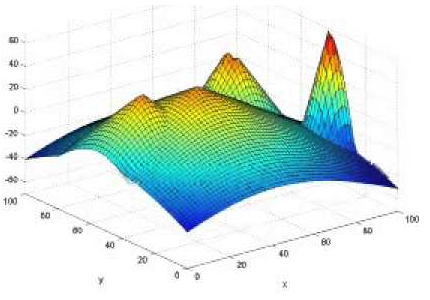
\includegraphics[scale=0.5]{images/moving_peak.png}
	\label{fig:moving_peaks}{\\Fonte: \citeonline{moving_peak_1999}.}
\end{figure}

\subsection{\textit{Ocillating Peaks}}
\label{sec:ocillating_peaks}

O \textit{benchmark} de oscilação de picos (\textit{ocillating peaks}) é baseado no de movimentação de picos, porem foi desenvolvido para algoritmos evolutivos com utilização de memória.

É uma combinação linear entre duas funções em que o peso delas se alteram ao longo do tempo, portanto, a função $G$, começa em $g_1$, passa para $g_2$, depois volta para $g_1$ e assim sucessivamente. Em outras palavras, o máximo absoluto de $G$ oscila entre dois pontos $g_1$ e $g_2$. As funções que representam as alteração da função $G$ estão representadas na Equação \ref{eq:ocillating_peak_alterations}, em que, $\lambda (t)$ representa a oscilação da função, $n$ é a soma das picos das duas funções que compõem a combinação linear e $m$ é o número de dimensões.

\begin{equation}
\label{eq:ocillating_peak_alterations}
\begin{split}
& \delta \in N(0,1) \\
& \lambda (t) = \frac{\cos{\frac{2\pi t}{100\delta}} +1}{2} \\
& g_1(\vec{x}) = \sum_{i=1}^{n/_2} \frac{H_i}{1+W_i \sum_{j=1}^{m} (x_j - X_j(t))^2} \\
& g_2(\vec{x}) = \sum_{i=n/_2+1}^{n} \frac{H_i}{1+W_i \sum_{j=1)}^{m} (x_j - X_j(t))^2} \\
& G(t,\vec{x}) = \lambda (t) g_1(\vec{x}) + (1-\lambda (t))g_2(\vec{x})
\end{split}
\end{equation}

\subsection{\textit{Shaky Ladder Hyperplane-defined Functions}}
\label{sec:df1_generator} 

\textit{Shaky Ladder Hyperplane-defined Functions} \cite{rand2005shaky}

\subsection{Gerador de Problemas testes para Ambientes não Estacionários}
\label{sec:df1_generator}

O Gerador de Problemas testes para Ambientes não Estacionários (DF1) foi utilizado para gerar ambientes, tais como o mostrado na Figura \ref{fig:problem_generator} proposto por Morrison e Jong \cite{morrison1999test}. Este gerador é capaz de criar um número especificado de pontos ótimos em duas dimensões utilizando a Equação \ref{eq:problem_generator} 

\begin{figure}[!htb]
	\caption{Gráfico que representa os ambientes gerados pelo Gerador de Problemas testes para Ambientes não Estacionários}
	\centering
	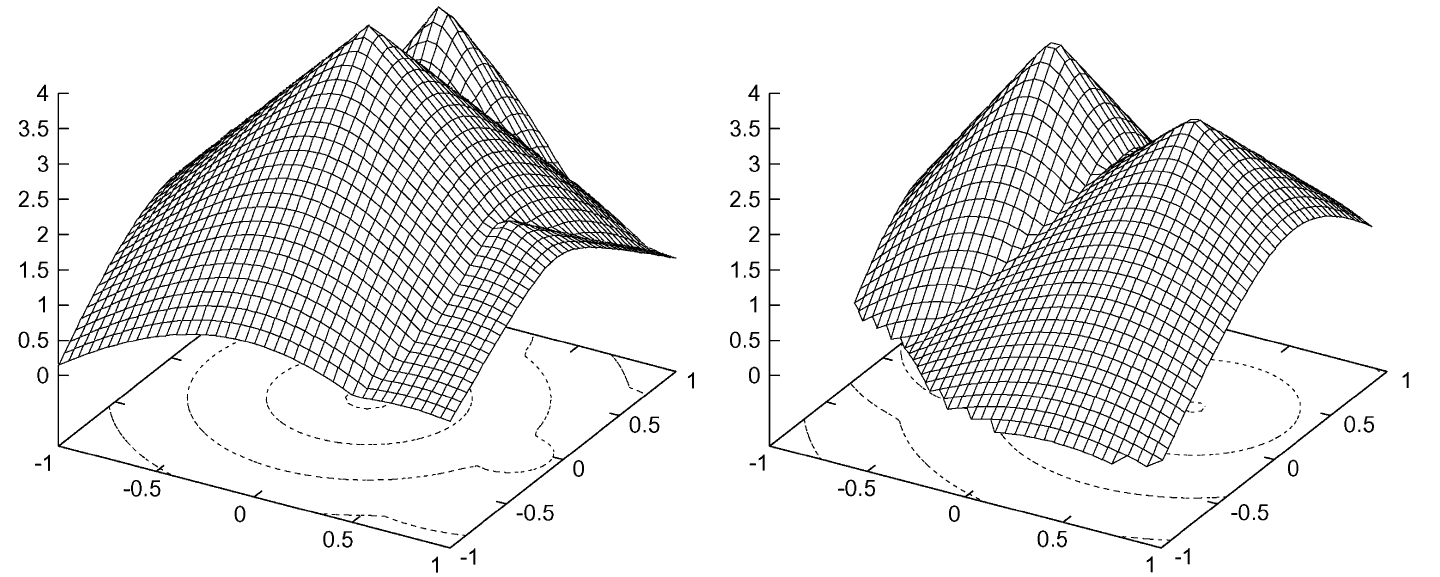
\includegraphics[scale=0.31]{images/bm_generator.png}
	\label{fig:problem_generator}{\\Fonte: \citeonline{morrison1999test}.}
\end{figure}

\begin{equation}
\label{eq:problem_generator}
\begin{split}
& f(X,Y) = \max_{i=1,N}\left[H_i - R_i . \sqrt{(X - X_i)^2 + (Y - Y_I)^2}\right] \\
& H_i \in [H_{base}, H_{base} + H_{range}] \\
& R_i \in [R_{base}, R_{base} + R_{range}]
\end{split}
\end{equation}

\noindent Em que $N$ representa o número de pontos ótimos a serem gerados, $(X,Y)$ representa sua posição, $H_i$ representa sua altura e $R_i$ representa sua inclinação. o limite da altura e inclinação são apresentados na Equação \ref{eq:problem_generator}. Nesse sistema variam suas posições, formas e alturas. A alturas varia entre um valor máximo e mínimo, criando assim um perfil de dente de serra, enquanto a altura é representada graficamente. O \textit{fitness} de cada ponto da superfície é atribuído a altura máxima de todos os pontos ótimos.

Embora o número de pontos ótimos presente não pode ser alterado uma vez que o ambiente tenha sido inicializado, a combinação de mudança alturas e posições faz com uma solução ótima fique temporariamente obscura em relação ao vizinhos, assim da a impressão que alguns pontos desaparecem e ressurgem. O dinamismo do ambiente pode ser especificado por um parâmetro $A$ que varia de [0, 4]. A direção de cada etapa é escolhido aleatoriamente para coordenadas espaciais, com passos que podem colocar um pico fora dos limites das variáveis. A direção da mudança na variáveis de altura e inclinação são escolhidas aleatoriamente inicialmente e continuam nessa direção até exceder o intervalo.